
\overlays{2}{%
  \begin{slide}{Das Fahrerinterface}
      \begin{minipage}{7.0cm}
        \untilSlide*{1}{%
          Gr�nde f�r einen PDA:
          \begin{itemize}
          \item Gen�gend Rechenleistung (Hochsprachen)
          \item Display (Warnhinweise)
          \item Interaktion (Einstellungen, Routing, etc.)
          \end{itemize}
        }
      \fromSlide*{2}{%
        Gr�nde f�r \emph{diesen} PDA
        \begin{itemize}
          \item Display
          \item Rechenleistung
          \item Linux (Multitasking, Programmierung)
        \end{itemize}
      }
    \end{minipage}
    \begin{minipage}{3cm}
      \begin{center}
        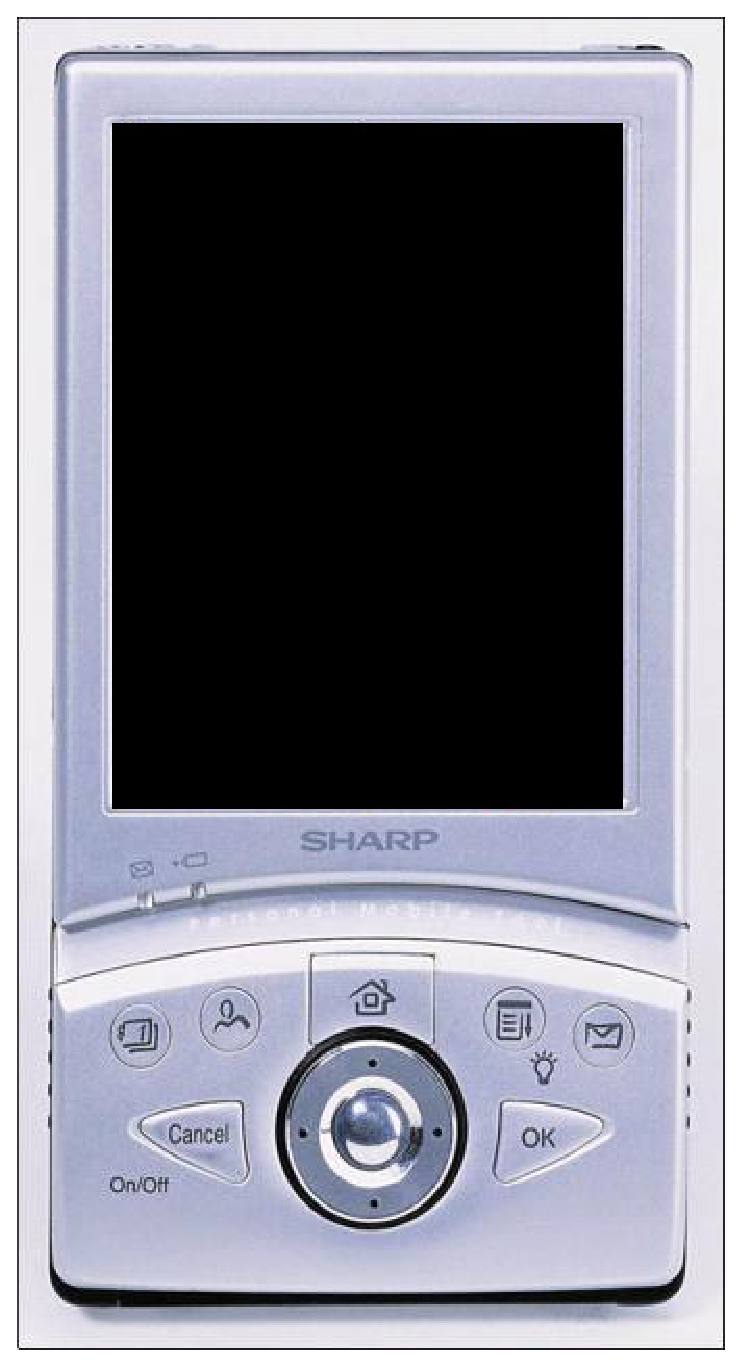
\includegraphics[width=3cm]{zaurus.eps}
      \end{center}
    \end{minipage}
  \end{slide}
}


% ============================================================


\overlays{2}{
  \begin{slide}{DPI aus Entwicklersicht}
    \untilSlide*{1}{
      \begin{center}
        Informal: Kommunizierende Automaten\\
        
\includegraphics[width=9cm, angle=-90]{zustaende.eps}

      \end{center}
    }
    \fromSlide{2}{
      Vaterklasse \texttt{Driver} f�r alle Treiber
      \begin{itemize}
      \item GUI ruft \texttt{Blinken()} des Treibers auf.
      \item \texttt{send(Message)}: Versenden von \emph{Nachrichten}.
      \item \texttt{receive(Message)}: Empfang von Nachrichten.
      \end{itemize}
    }
  \end{slide}
}


% ============================================================


  \begin{slide}{Weg der Nachricht durch das DPI}
    \begin{itemize}
    \item \texttt{Driver.send()} �berpr�ft die Nachricht
    \item \texttt{message\_dispatcher.send()} sendet auf passendem
      \texttt{bus\_manager} heraus $\to$ Indirektion
    \item \texttt{bus\_manager.send()} sendet auf passendem
      \texttt{bus} heraus $\to$ Indirektion
    \end{itemize}
  \end{slide}